\section{Geocodierung}
\label{geocodierung}
Ein grosser Vorteil der Google Fusion Tables ist die automatische 
\gls{Geocodierung} von Standortdaten. Sobald eine neue Zeile zu einer Tabelle hinzugefügt wird, werden alle Zellen vom Typ \emph{Location} einem eindeutigen Standort auf der Karte zugewiesen. Ist dies nicht möglich, da beispielsweise eine Adresse in mehreren Orten vorkommen kann, bleibt die Zelle gelb hinterlegt.
 
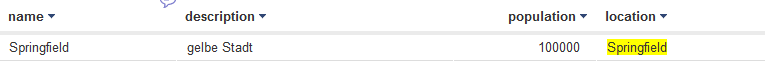
\includegraphics[scale=0.75]{images/geocoding_failed.png}

Diese geocodierten Standorte werden in der Tabelle hinterlegt sind aber mit den SQL API nicht selektierbar. Man müsste also für jede Zeile die man als Resultat erhält die Geocodierung manuell vornehmen, was sich negativ auf die Ladezeit der Karte auswirken würde.
Es gibt verschiedene Dienste, welche eine solche Geocodierung von Standortdaten anbieten. Die meisten davon haben aber eine Begrenzung der möglichen Anfragen pro Tag.

\begin{longtable}{|l|p{1.9cm}|p{7.3cm}|}
\hline 
\textbf{Anbieter} & \textbf{Anfragen pro Tag} & \textbf{URL} \\ 
\hline 
Google Maps Geocoding API & 2500 & \url{https://developers.google.com/maps/documentation/geocoding/?hl=de} \\ 
\hline 
Yahoo! PlaceFinder API & 50000 & \url{http://developer.yahoo.com/geo/placefinder/} \\ 
\hline 
MapQuest Geocoding API & keine Begrenzung & \url{http://developer.mapquest.com/web/products/dev-services/geocoding-ws} \\ 
\hline 
\end{longtable} 

Wie man sieht erreicht man mit diesen Diensten beim Arbeiten mit grossen Datenmengen schnell die Grenzen.

\subsection{Bug beim Geocoding von neuen Datensätzen}
\label{geocodierung-bug}
\todo[inline]{Geocoding-Bug beschreiben}